\section{Progettazione}

\subsection{Design Persona}

Partendo dalla risorsa consigliata nel corso (\textit{Desining for Emotion} di Aaron Walter), abbiamo descritto la personalità di partenza per sviluppare il prodotto:
\begin{itemize}
    \item \textbf{Brand name}: a questo punto il nome del brand è noto, ovvero \textit{Penny Wise};

    \item \textbf{Overview}: abbiamo scelto di usare come \textit{mascotte} Paperon De Paperoni, infatti, dato che si tratta di un progetto universitario, abbiamo la possibilità di partire da un personaggio fantastico molto noto, senza doverci preoccupare di copyright;

    \item \textbf{Brand traits}:
        \begin{itemize}
            \item Risparmiatore: la caratteristica che spicca del personaggio è il suo amore per il risparmio;

            \item Familiare, ma non scontato (forse anche un po' scontato);

            \item Laborioso, ma non \textit{workahoolic}: è partito avendo solo un piccone e deve la sua fortuna al suo duro lavoro;

            \item Scherzoso, ma non trasandato: si tratta del personaggio di un fumetto comunque legato all'infanzia di ognuno di noi;

            \item Oculato: si tratta del papero pià ricco di tutta Paperopoli!
        \end{itemize}
    
    \item \textbf{Personality map}:
        \begin{center}
            \begin{tikzpicture}
                \begin{axis}[
                    axis lines = middle,
                    xlabel = {Dominant},
                    ylabel = {Friendly},
                    xmin = -10, xmax = 10,
                    ymin = -10, ymax = 10,
                    xtick = {-10,-5,...,10},
                    ytick = {-10,-5,...,10},
                ]
					\addplot [
						color=black,
						mark=*,
						only marks,
					] coordinates {
					(8, -2)
				} node[below] {$P$};
                \end{axis}
                
            \end{tikzpicture}
        \end{center}

    
    \item \textbf{Voice}: 
		\begin{itemize}
			\item Non viene raggiunto un obiettivo di risparmio: "Paperone è
				infastidito e incoraggia a migliorare";
				
			\item Se raggiungi l'obiettivo di risparmio: "Paperone ti guarda 
				dall'alto del suo gruzzolo di monete, e ti incoraggia a 
				continuare";

			\item Se il conto è in rosso: "Paperone è furioso e ti invita a 
				rimediare!";
		\end{itemize}
    
    \item \textbf{Copy examples}: potrebbe cambiare il logo del sito in base
		alla situazione del progetto, oppure potrebbe comparire una vignetta;
    
    \item \textbf{Visual lexicon}:
		\begin{itemize}
			\item \textbf{Colori}: giallo e blu scuro;
			\item \textbf{Contorni}: arrotondati;
			\item \textbf{Ombre}: assenti;
			\item \textbf{Font}: \textit{Sans-Serif Arial};
		\end{itemize}
    
    \item \textbf{Engagement methods}:
		\begin{itemize}
			\item \textbf{Feedback}: ad ogni azione corriponde una notifica, in
				modo tale che l'utente abbia sempre un riscontro;

			\item \textbf{Design pulito e intuitivo}: l'utente deve essere in
				grado di capire cosa fare senza dover leggere alcun manuale;

			\item \textbf{Psicologia dei colori}: sono utilizzati dei colori
				accattivanti che richiamano il personaggio scelto;
		\end{itemize}
\end{itemize}

\subsection{Palette}

I colori principali della palette di \textit{Penny Wise} sono il giallo 
(\texttt{\#F4DF57}) e il blu molto scuro (\texttt{\#202630}): il giallo richiama 
il nome del prodotto, ovvero \textit{penny}, che si riferisce alle monete, 
trasmette ottimismo, energia e vitalità; mentre il blu scuro è scelto per 
esaltare il giallo, senza che quest'ultimo debba essere aggressivo.

\subsection{Accessibilità}

L'accessibilità è un indice di qualità del sito, pertanto è stata fin da subito
un proposito imprescindibile che ha guidato la fase di progettazione e le
successive. Per quanto siamo incorsi in alcune difficoltà. Di seguito sono
riportate le misure adottate per garantire un'esperienza di utilizzo ottimale
per tutti gli utenti.

\subsubsection{Orientamento dell'utente}

L'utente deve essere in grado di costruire una mappa mentale durante
l'esplorazione del sito, in questo modo evita situazioni di disorientamento o
sovraccarico cognitivo. Per questo motivo, prima di sviluppare la gerarchia
delle pagine, abbiamo creato una mappa concettuale che ci ha permesso di 
organizzare i contenuti in modo chiaro e coerente. Inoltre, sono adoperati
accorgimenti per aiutare gli utenti che navigano le pagine mediante
\textit{screen-reader}.

\begin{figure}[H]
	\centering
	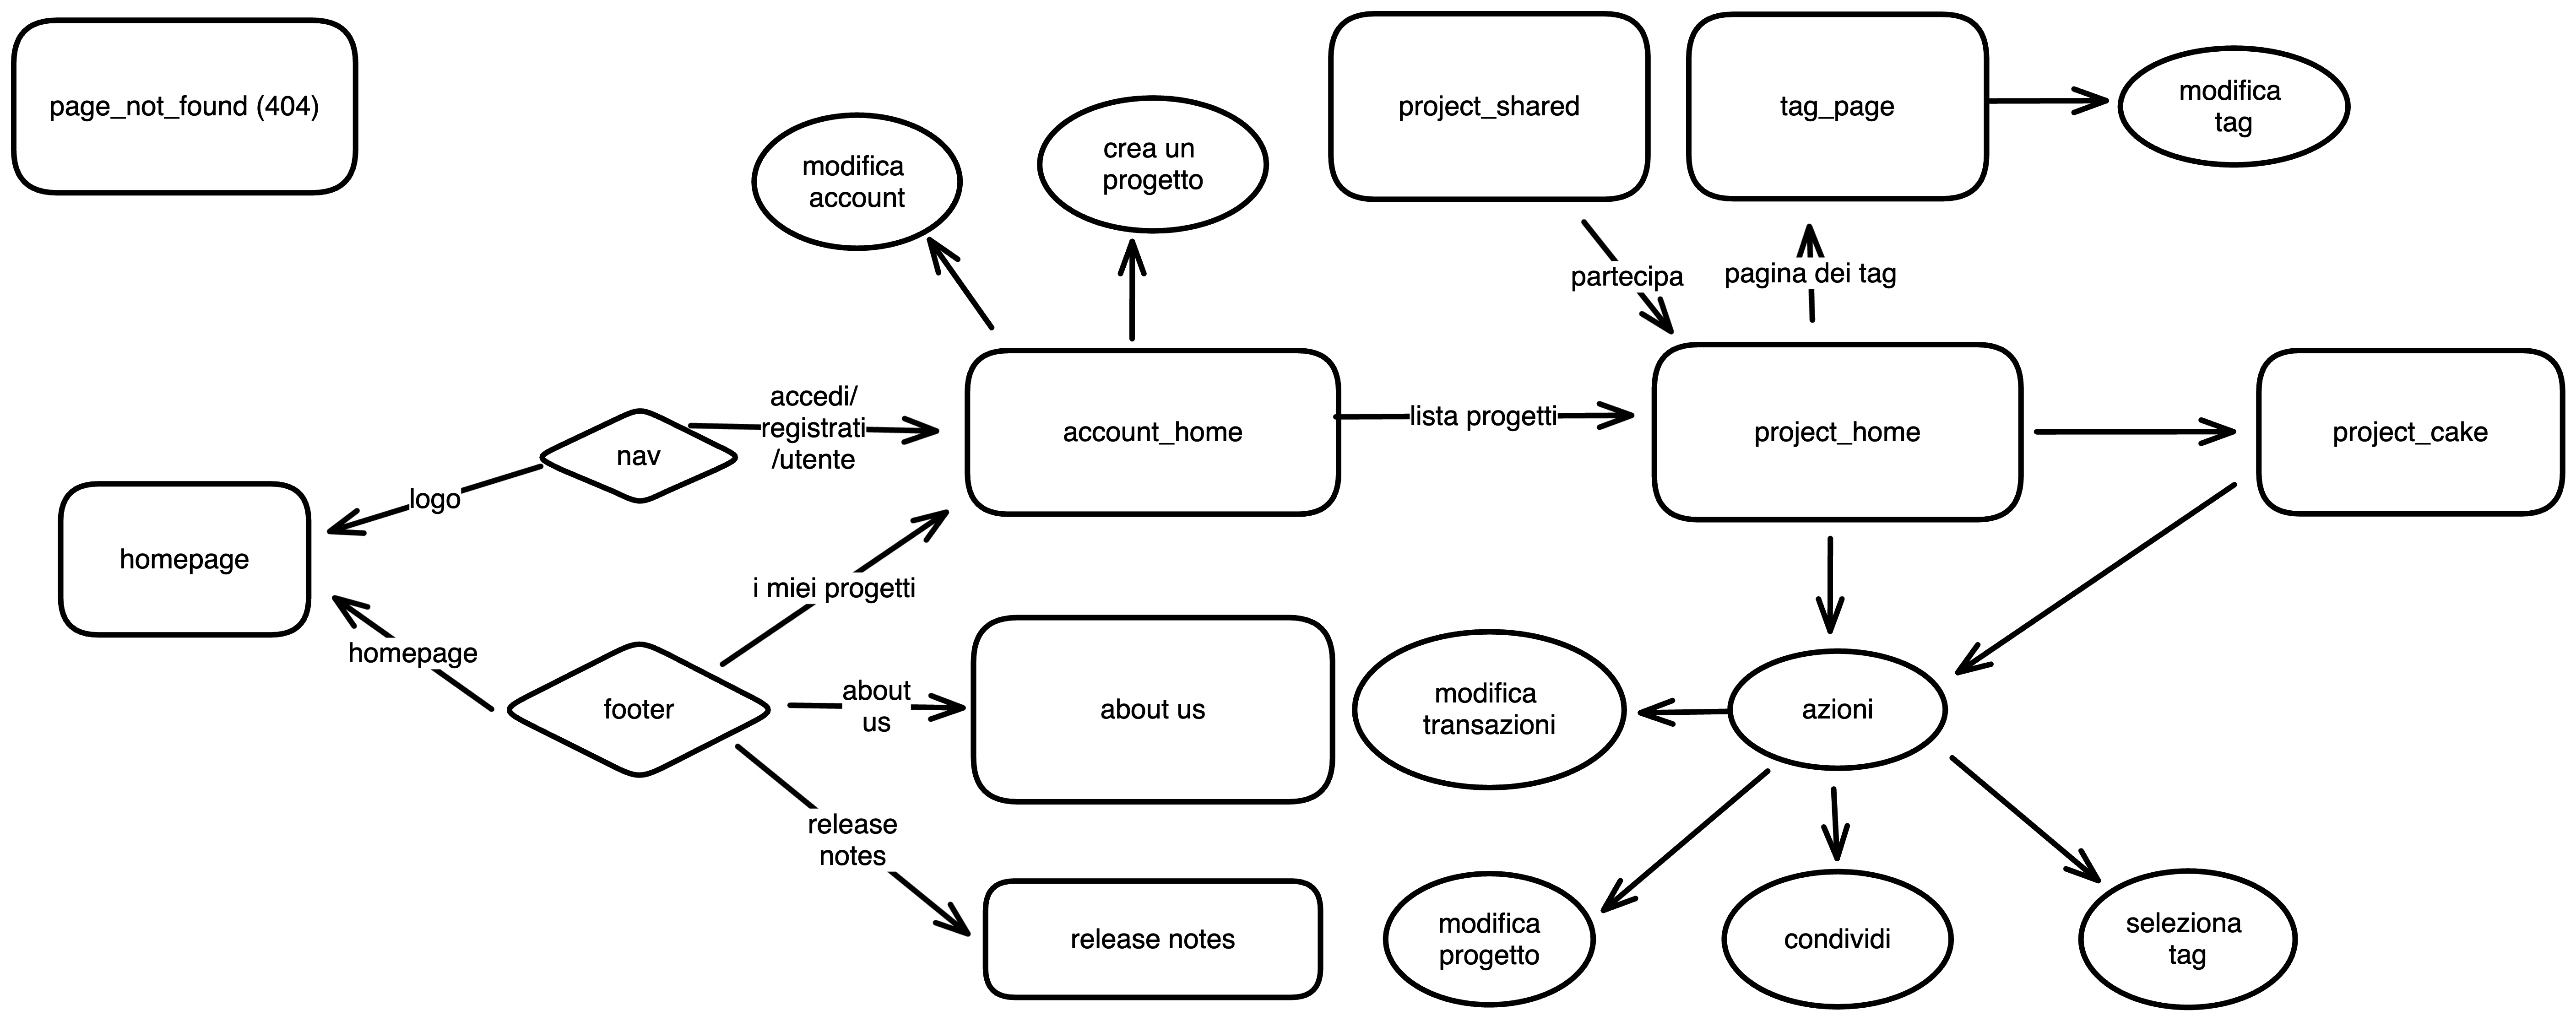
\includegraphics[width=0.8\textwidth]{figures/sitemap.png}
	\caption{Mappa concettuale del sito}
\end{figure}

\subsubsection{Colori}

I colori sono stati scelti appositamente con un contrasto elevato tra loro in
modo da garantire una buona leggibilità anche da parte di utenti con deficit
parziale della vista, infatti è stato rispettato lo standard WCAG AA.

\subsubsection{Responsive layout}

Il sito è stato progettato per adattarsi a qualsiasi dispositivo, in modo da
garantire un'esperienza di utilizzo ottimale sia da desktop che da mobile. Per
questo motivo, sono stati adottati layout flessibili e fluidi, in modo da
garantire una buona leggibilità e usabilità indipendentemente dalla dimensione
dello schermo o dalle preferenze dell'utente.

\subsection{Struttura del sito}

Il sito è organizzato in una struttura gerarchica per conciliare facilità di utilizzo e organizzazione delle informazioni in modo ordinato e preciso. I contenuti sono suddivisi secondo uno schema organizzativo per argomento di seguito sono descritte le singole pagine:

\begin{itemize}
    \item \textbf{Home}: si tratta della pagina di accesso al sito. Nell'area sicura sono presenti l'identità (logo e nome del servizio) e il menu. Scorrendo viene fornita un'introduzione al servizio, ovvero alle funzionalità offerte dal sito;

    \item \textbf{About Us}: contiene una breve descrizione delle motivazioni
		che hanno portato allo sviluppo del prodotto, oltre ad una breve
		introduzione delle persone che hanno realizzato \textit{Penny Wise};

    \item \textbf{Release Notes}: \textit{timeline} dei progressi del progetto;

    \item \textbf{Account Home}: contiene le informazioni dell'Utente Registrato, inoltre da questa pagina è possibile accedere al form per modificare tali informazioni. Infine, è presente la lista dei progetti e le funzionalità di gestione di un progetto;
    
    \begin{itemize}
        \item \textbf{Project Home}: contiene le informazioni di un progetto, ovvero il nome e la descrizione di esso. Mostra anche le transazioni contenute nel progetto, i partecipanti e i tag del progetto. Infine è mostrato un grafico interattivo che mostra l'andamento delle spese del progetto nel periodo di tempo desiderato;
        
        \begin{itemize}
            \item \textbf{Project Cake}: contiene le medesime informazioni della pagina \textit{Project Home}, però il grafico dell'andamento delle spese viene sostituito con un grafico a torta che mostra la proporzione dei tag rispetto alle spese. Si noti che anche in questo caso è possibile modificare il periodo di tempo considerato;

            \item \textbf{Tag Page}: questa pagina mostra l'elenco dei tag associati ad un progetto e ne permette la gestione, ovvero la creazione, la modifica o l'eliminazione.
        \end{itemize}
    \end{itemize}

    \item \textbf{Project Shared}: si tratta della pagina per effettuare
		l'accesso ad un progetto condiviso. Vi si accede tramite il link di
		condivisione del progetto;
\end{itemize}

